\section{Concepto}

Antes debemos de plantearnos que es un instrumento financiero, pues bien, \textit{un instrumento financiero es un contrato que da ligar a un activo financiero para una empresa y, simultáneamente, a un pasivo financiero o a un instrumento de patrimonio para otra empresa.}

Como ejemplo, podemos destacar una gran cantidad, pero nos centraremos en 3 que serán los que trataremos en este capítulo:
\begin{itemize}
    \item Créditos a terceros: Préstamos y créditos financieros concedidos, incluidos los surgidos de la venta de activos no corrientes.
    \item Valores representativos de deuda de otras empresas adquiridos: obligaciones, bonos y pagarés.
    \item Instrumento de patrimonio de otras empresas adquiridos: acciones, participaciones en instituciones de inversión colectiva y otros instrumentos de patrimonio.
\end{itemize}


Dentro de esta también se regula la problemática relatica a las \textit{acciones propias}, considerando que \textit{surgirá como un activo o un pasivo financiero en operaciones que se vayan a liquidar entregando instrumentos de patrimonio propio}, es decir acciones propias de la empresa, cuando de los mismos estemos considerando que son mecanismos de pago.

La empesa reconocerá un activo financiero cuando se convierta en una parte obligada del contrato o negocio jurídico.

Si los elementos suponen un derecho de cobra, y no derivan de una relación contractual, sino que tienen su origen en un requerimiento legal o en actividades de fomento por parte de las Administraciones Públicas, \textit{no se consideran activos financieros}.

Las cuentas a tener en cuenta en este apartado, son:
\begin{itemize}
    \item 24 Inversiones financieras a largo plazo en partes vinculadas.
    \item 25 Otras inversiones financieras a largo plazo.
    \item 26 Fianzas y depósitos constituidos a largo plazo.
    \item 29 Deterioro del valor del inmovilizado.
    \item 43 Clientes.
    \item 44 Deudores.
    \item 49 Deterioro de valor de créditos comerciales y provisiones a corto plazo.
    \item 53 Inversiones financieras a corto plazo en partes vinculadas.
    \item 54 Otras inversiones financieras a corto plazo.
    \item 55 Otras cuentas no bancarias.
    \item 57 Tesorería.
    \item 59. Deterioro valor de instrumentos financieros a corto plazo y activos no corrientes.
\end{itemize}

\section{Clasificación AF}

Dependiendo dee su naturaleza, los activos financieros se clasifican en:
\begin{itemize}
    \item Activos financieros a coste amortizado.
    \item Activos financieros a valor razonable con cambios en el partrimonio neto \textit{AFVRPN}.
    \item Activos financieros a coste.
    \item Activos financieros a valor razonable con cambios en la cuenta de pérdidas y ganancias \textit{AFVRPYG}.
\end{itemize}

En términos generales, los activos financieros deben de valorarse a valor razonable con cambios en la cuenta de pérdidas y ganancia, con la excepción de:
\begin{itemize}
    \item Las invesiones valoradas a coste o inversiones en el patrimonio del grupo o asociadas, deben de ser clasificados como \textit{Activos financieros a coste}.
    \item Los activos financieros que tienen una estructura común a la del préstamo, es decir, del mismo se deriva una estructura de flujos de efectivo similar a la de amortización e intereses financieros, y además, que la empresa tenga la intención de mantenerlo para recibir esos flujos de efectivo, se clasificarán dentro de la categoría de \textit{Activos a coste amortizado}.
    \item Cuando la gestión del activo consista en recibir flujos de efectivo de un acuerdo básico de préstamos (amortización e intereses), pero también se pueda acordar su enajenación antes del vencimiento de los mismos. Estos se valoran como \textit{Activos financieros a valor razonable con cambios en el patrimonio neto [AFVRPN]}
\end{itemize}

Cuando no sea ninguna de las condiciones anteriores, el activo se valorará como \textit{Activos financieros a valor razonable con cambios en la cuenta de pérdidas y ganancias [AFVRPYG]}.

Ahora vamos a tratar los AF que pueden ser considerados en estas catergorías de forma específica.

\begin{enumerate}
    \item Activos financieros a coste amortizado.
    \begin{itemize}
        \item Créditos por operaciones comerciales: se originan por la venta de bienes y la prestación de servicios por operaciones de tráfico.
        \item Créditos por operaciones no comerciales: son aquellos AF, que no siendo isntrumentos de patrimonio ni derivados, no tienen origen comercial y cuyos cobros son de cuantía determinada o determinable, que procedes de \textit{operaciones de préstamo o crédito concedidos por la empresa}.
    \end{itemize}


    Se incluirán en esta categoría, incluso cuando esté admitido a negociación en un mercado organizado, si la empresa mantiene la inversión con el objetivo de percibir los flujos de efectivo derivados de la ejecución del contrato y las condiciones contractuales del AF dan lugar, en fechas específicas, a flujos de efectivo que son únicamente cobros de principal e intereses (SCPI).

    A continuación, definimos que entendemos por modelo de negocio y por las características del activo (SCPI):
    \begin{enumerate}
        \item Modelo de Negocio (MN): modelo que la empresa sigue en relación con la gestión del activo. Algunos aspectos a considerar son:
        \begin{itemize}
            \item Una empresa tiene varios modelos de negocio para gestionar sus carteras de activos.
            \item ¿Es posible clasificar una cartera de activos a coste amortizado aunque se vendan antes de los que se establece en el contrato? Sí es posible. \textit{La gestión de un grupo de activos financieros para obtener sus flujos contractuales no implica que la empresa haya de mantener todos los instrumentos hasta su vencimiento}.
            \item ¿Qué criterio es necesario tener en cuenta para decidir si una cartera de activos a coste amortizado cumple el modelo de negocio? Es necesario analizar \textit{frecuencia, importe y el calendario de las ventas de ejercicio anteriores, motivos de las ventas y las expectativas en relación con la actividad de ventas futuras}.
            \item Si se detectan incrementos de frecuencias en ventas, la empresa debe de explicar la razón y demostrar que no hay un cambio en el modelo de negocio. No se establece el límite cuantitativo específico para determinar los cambios en el modelo de negocio.
        \end{itemize}
        \item Características del Activo (SCPI): La condición se cumple si \textit{las condiciones contractuales del activo financiero dan lugar a flujos de efectivo que son únicamente cobros de principal e intereses sobre el importe del principal pendiente}. Cuando se cumplen las condiciones anteriores, los activos deben de clasificarse como \textit{Activos financieros a coste amortizado}. Cuando cumplan las condiciones del SCPI, pero no atienda a un modelo de negocio que viene desarrollando la empresa, se clasificarán como \textit{Activos financieros a valor razonable con cambios en el patrimonio neto[AFVRPN]}.
    \end{enumerate}

    \item Activos financieros a valor razonable con cambios en el patrimonio neto [AFVRPN].
    Se incluirán en esta categoría cuando las condiciones contractuales del activo financiero den lugar a flujos de efectivo que son únicamente cobros de principal e intereses sobre el importe del principal pendiente, \textit{y no se mantenga para negociar ni proceda clasificarlo en la categoría regulada en el apartado 2.2 de esta norma}.
    También se incluirán en esta categoría las inversiones de patrimonio para las que se haya ejercitado la opción irrevocable (no se mantengan para negociar, ni deban valorarse al coste).

    \item Activos financieros a coste.
    
    En esta categoría se incluyen:

    \begin{enumerate}
        \item Inversiones en el patrimonio de empresas del grupo y asociadas.
        \item Restantes inversiones en instrumentos de patrimonio sin valor razonable por referencia a valor cotizado.
        \item Los activos financieros híbridos cuyo VR no puede estimarse de manera fiable.
        \item Las aportanciones realizadas como consecuencia de un contrato de cuentas de participación y similares.
        \item Préstamos participativos cuyos interes tengan un carácter contingente.
        \item Cualquier otro activo financiero, cuando no sea posible obtener una estimación fiable de su valor razonable.
    \end{enumerate}

    \item Activos financieros a valor razonable con cambios en la cuenta de pérdidas y ganancias [AFVRPYG].
    
    Se debe de incluir en esta categoría salvo que proceda su clasificación en alguna de las restantes categorías.

    En cualquier caso, los activos financieros mantenidos para negociar se incluirán obligarioriamente en esta catergoría.

\end{enumerate}

A efectos de catalogar lo que se entiende por negociación, consideramos las compras y ventas con el objetivo de generar una ganacia por las fluctuaciones a c/p. El activo \textit{adquiere esta condición} cuando:

\begin{itemize}
    \item Se origine o adquiera con el propósito de venderlo en el corto plazo.
    \item Forme parte en el momento de su reconocimiento inicial de una cartera de instrumentos financieros identificados y gestionados conjuntamente.
    \item Sea un instrumento financiero derivado
\end{itemize}

Los que se mantengan para negociar, ni se valoren al coste, la empresa puede realizar \textit{elección irrevocable}, en el momento de su reconocimiento inicial, de presentar los cambios posteriores en el VR directamente en el PN.

Por último, un activo se puede incluir en esta categoría para reducir las asimetrías contables. Esta opción hace referencia a la valoración de los activos de manera conjunta, aunque alguno de sus componentes se pueda valorar de manera separada.

La siguiente Figura \ref{fig:Acciones} muestra la clasificación de las acciones, en base a los siguientes criterios:

\begin{itemize}
    \item Exitencia de un modelo de negocio o SCPI. Si no se cumple no es posible clasificar el instrumento de patrimonio como \c{Activos financieros a coste amortizado}.
    \item Existencia o no de VR. Si no, solo puede valorarse a \c{coste}.  
    \item Intención o no de negociar. Si esta condiciones se cumple, se valorará a \c{valor razonable con cambios en la cuenta de pérdidas y ganancias}, mientras que si no se cumple debemos de valorar a \c{valor razonable con cambios en el patrimonio neto}.
\end{itemize}

\begin{figure}[H]
    \centering
    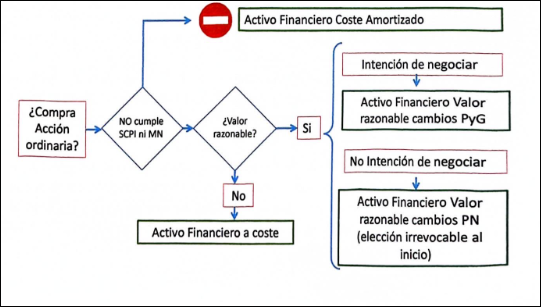
\includegraphics[width=0.8\textwidth]{images/clasacc.png}
    \caption{Clasificación de las acciones}
    \label{fig:Acciones}
\end{figure}

De la misma manera, la Figura \ref{fig:Deuda} muestra la clasificación de la deuda, en base a los mencionados anterirmente.

\begin{figure}[H]
    \centering
    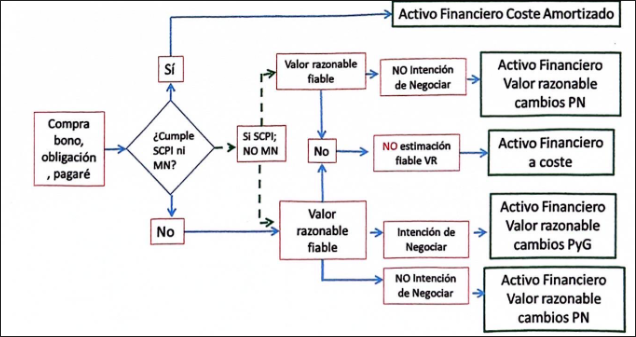
\includegraphics[width=0.8\textwidth]{images/deuda.png}
    \caption{Clasificación de la deuda}
    \label{fig:Deuda}
\end{figure}

\subsection*{\textcolor{blue}{Ejemplo 2}}

La empresa CHOTIS, S.A. realiza diferentes adquisiciones de instrumentos de patrimonio y de deuda, con las siguientes características:

\begin{enumerate}
    \item Adquisición de 100 acciones cotizadas en mercado activo, donde se plantean dos opciones:
    \begin{enumerate}
        \item La empresa tiene intención de negociar.
        \item La empresa tiene intención de mantenerlas a largo plazo.
    \end{enumerate}
    \item Adquisición de 100 obligaciones cotizadas en mercado activo, donde se plantean dos opciones:
    \begin{enumerate}
        \item La empresa tiene intención de mantener el modelo de negocio, esperar a vencimiento y recibir los flujos de efectivo contractuales.
        \item La empresa tiene intención de especular o negociar con las mismas en el corto plazo y no espera recibir los flujos de efectivo contractuales.
    \end{enumerate}
    \item Adquisición de 100 acciones no cotizadas en mercado activo, donde no es posible determinar un valor razonable fiable.
    \item Adquisición de 100 obligaciones no cotizadas en mercado activo, donde se plantean dos opciones:
    \begin{enumerate}
        \item La empresa tiene intención de mantener el modelo de negocio, esperar a vencimiento y recibir los flujos de efectivo contractuales.
        \item La empresa tiene intención de especular o negociar con las mismas en el corto plazo y no espera recibir los flujos de efectivo contractuales.
    \end{enumerate}
    En ambos casos no es posible disponer de un valor razonable fiable.
\end{enumerate}

La respuesta a este ejercicio se muestra en la Cuadro \ref{tab:Chotis}.


\begin{table}
    \centering 
    % \begin{tabular}{|p{3cm}|p{3cm}|p{3cm}|p{3cm}|p{3cm}|}
    \begin{tabularx}{\textwidth}{|X|X|X|X|X|}
        \hline 
        Categorías & Compra 100 acciones, cotizadas en un mercado activo. & Compra 100 obligaciones, cotizadas en un mercado activo. & Compra 100 acciones, no cotizadas en un mercado activo & Compra 100 obligaciones, no cotizadas en un mercado activo. \\
        \hline
        Modelo de negocio / Cobros principal e intereses & No modelo de negocio y no SCPI- Existe VR fiable. Tenemos dos opciones: \begin{itemize}
            \item Intención de negociar.
            \item No negociar.
        \end{itemize}& 
        \begin{itemize}
            \item Opción A: La empresa tiene intención de percibir flujos de efectivo y MN.
            \item Opción B: Sin MN y sin intención de percibir flujos de efectivo. Intención de negociar.
        \end{itemize} & 
        No MN y no SCPI. Intención de negociar. No es posible estimar un VR fiable & 
        \begin{itemize}
            \item Opción A: No puede estimarse un VR fiable, pero si hay SCPI y MN.
            \item Opción B: Carácter inversión especulativa sin VR.
        \end{itemize} \\
        \hline
        \hline
        AVRF (PyG) & \ding{51} (A) & \ding{51} (B) & \ding{55} & \ding{55} \\
        \hline
        Activos a coste amortizado & \ding{55} & \ding{51}(A) & \ding{55} & \ding{51}(A) \\
        \hline
        Activos a coste & \ding{55} & \ding{55} & \ding{51} & \ding{51}(B) \\
        \hline
        AVRF (PN) & \ding{51}(B) & \ding{51}(A) & \ding{55} & \ding{55} \\
        \hline
    \end{tabularx}
    \caption{Clasificación de activos financieros de la Chotis S.A.}
    \label{tab:Chotis}
\end{table}

% \begin{table}
%     \centering
%     \begin{tabular}{|p{3cm}|p{3cm}|p{3cm}|p{3cm}|p{3cm}|}
%         \hline
%         AVRF (PyG) & \ding{51} (A) & \ding{51} (B) & \ding{55} & \ding{55} \\
%         \hline
%         Activos a coste amortizado & \ding{55} & \ding{51}(A) & \ding{55} & \ding{51}(A) \\
%         \hline
%         Activos a coste & \ding{55} & \ding{55} & \ding{51} & \ding{51}(B) \\
%         \hline
%         AVRF (PN) & \ding{51}(B) & \ding{51}(A) & \ding{55} & \ding{55} \\
%         \hline
%     \end{tabular}
%     \caption{Clasificación de activos financieros de la Chotis S.A.}
%     \label{tab:Chotis2}
% \end{table}

Como se ha señalado a lo largo de este capítulo, es necesario identificar, en primer lugar, si se cumple el modelo de negocio y el modelo SCPI. Además, se debe indicar si el activo tiene un valor razonable y éste es fiable, determinando si la intención es negociar con los mismos. Con estas premisas:

\begin{enumerate}
    \item Para el caso 1:
    \begin{itemize}
        \item Si no se cumplen el SCPI ni el modelo de negocio, pero existe un valor razonable fiable, la clasificación depende de la intención de la empresa.
        \begin{itemize}
            \item Sin intención de negociar: AFVRPN.
            \item Con intención de negociar: AFVRPYG.
        \end{itemize}
    \end{itemize}

    \item Para el caso 2:
    \begin{itemize}
        \item Opción a): Si se cumplen el SCPI y el modelo de negocio, el instrumento de deuda se clasifica como activo a coste amortizado.
        \item Opción b): Si no se cumple ningún criterio, los instrumentos de deuda se clasifican como AFVRPYG.
    \end{itemize}

    \item Para el caso 3: 
    \begin{itemize}
        \item Los instrumentos de patrimonio no cotizados se clasifican como activos a coste.
    \end{itemize}

    \item Para el caso 4:
    \begin{itemize}
        \item Opción a): Con modelo de negocio y SCPI, se clasifican como activos a coste amortizado.
        \item Opción b): Sin valor razonable y siendo una inversión especulativa, se clasifican como activos a coste.
    \end{itemize}
\end{enumerate}

\c{Si no existiera un valor razonable fiable para los casos 1 y 2, se podrían clasificar como activos financieros a coste, según la NV9-2.4 f).}

\subsection*{\textcolor{blue}{Ejemplo 3}}

En este veremos otros activos financieros y como es su clasificación. Podemos verlo en la Cuadro \ref{tab:otrosAF}.


% \begin{enumerate}
%     \item \textbf{Acciones ordinarias.} No cumple con la condición de SCPI, es decir, de ellos no se puede establecer que exista un acuerdo de préstamos con devolución de principal. Partiendo de esto, debemos de ver si existe in VR y si es fiable o no. Si no existiera las acciones se deben de clasificar a coste. Si existiera un VR y se hace el reconocimiento inicial, se clasifica como AFVRPN. Si se tiene la intención de negociar, o cualquier otro caso se clasificará como AFVRPYG.
%     \item \b{Bono simple a tipo de interés fijo, o bono simple, en euros o con fecha de vencimiento determinada.}: \begin{itemize}
%         \item Inversión cumple con SCPI.
%         \item Si no lo vende hasta el vencimiento se clasifica como \c{Activos financieros a coste amortizado}, si es por el contrario se vende antes, se clasifica como \c{Activos financieros a valor razonable con cambios en el patrimonio neto}.
%         \item \b{Bono con remuneración referenciada a precios de acciones}
%     \end{itemize}
% \end{enumerate}

\begin{table}[H]
\centering
\begin{tabularx}{\textwidth}{|X|X|X|}
\hline
\textbf{Activo financiero} & \textbf{¿Cumple SCPI?} & \textbf{Se clasifica como...} \\ \hline
Acciones ordinarias & 
No cumple SCPI. El rendimiento (intereses) no refleja el valor temporal del dinero por el uso de un capital principal, y depende del valor de un título en el mercado. & 
• AFVR (PyG) si hay intención de negociar y el valor razonable es fiable. 
• AFVR (PN) si el valor razonable es fiable pero no hay intención de negociar. 
• A coste, si no cotizan en mercados activos. \\ \hline
Bono simple (interés fijo) & 
Cumple SCPI, se esperan flujos de efectivo contractuales con intereses que reflejan el valor temporal del dinero. & 
• AFVRC si se piensa negociar a corto plazo. 
• A coste amortizado, si se mantienen a vencimiento.
• A coste, si no cotizan en mercados activos. \\ \hline
Bono referenciado a acciones & 
No cumple SCPI. Intereses dependen de precios de acciones, no reflejan valor temporal del dinero. & 
• AFVR (PyG) si el valor razonable es fiable y hay intención de negociar.
• AFVR (PN) si no hay intención de negociar. \\ \hline
Derivados (forwards, opciones) & 
No cumple SCPI. Los beneficios están sujetos a cambios en el mercado. & 
• AFVR (PyG) con valor razonable fiable.
• A coste, si el valor razonable no es fiable. \\ \hline
Bono a perpetuidad & 
No cumple SCPI. No refleja valor temporal del dinero. & 
• AFVR (PN), si el valor razonable es fiable.
• A coste, si no existe un valor razonable fiable. \\ \hline
\end{tabularx}
\caption{Clasificación y análisis de diferentes tipos de activos financieros.}
\label{tab:otrosAF}
\end{table}

\subsection{Valoración inicial y posterior de los activos financieros}

El siguiente paso es determinar el proceso de valoración de las mismas. (Ver Figura \ref{fig:Valoracion}).

\begin{figure}[H]
    \centering
    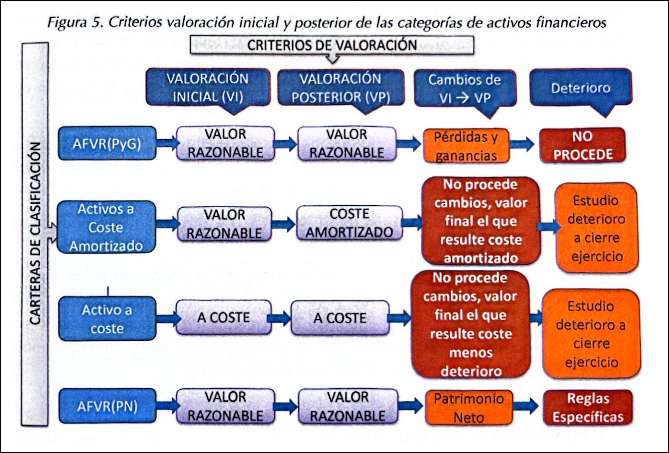
\includegraphics[width=0.9\textwidth]{images/cri_val.png}
    \caption{Valoración de los activos financieros}
    \label{fig:Valoracion}
\end{figure}

\section{AF con valoración posterior a coste amortizado}

\subsection{Valoración inicial}

Los activos incluidos en esta categoría se valorarán inicialmente por su VR, salvo evidencia en contrario. \c{Será el precio de la transacción, que equivladrá al VR de la contraprestación entregada más los costes de transacción.}

\subsection{Valoración posterior}

Se valorarán por su coste amortizado. Los intereses devengados se contabilizarán en la cuenta de Pérdidas y Ganancias, aplicando el tipo de interés efectivo (TIE).

Sabemos que la valoración posterior incluye alguno deterioros de valor en la mayoría de casos.

La primera parte del Marco Conceptual define el coste amortizado como \c{Importe al que inicalmente feu valorado un AF o un PF, menos los reembolsos del principal, más o menos la parte imputada en la cuenta de PyG, mediante la utilización del tipo de interés efectivo, de la diferencia entre el importe inicial y el valor de reembolso en el vencimiento.}

De esta definición cabe destacar:
\begin{enumerate}
    \item + valoración inicial del instrumento.
    \item - los reembolsos del princial realizados.
    \item $\pm$ la imputación en resultados de la diferencia entre el valor inicial y el valor de reembolso al vencimiento.
    \item - las reducciones por deterioro de valor.
\end{enumerate}

\subsection*{\textcolor{blue}{Ejemplo 4}}

La entidad A concede un crédito el 1-1-2018 a la entidad B con las siguientes características:

\begin{itemize}
    \item Nominal: 1.000.000 €.
    \item Comisión de apertura (a cargo de la empresa A): 10.000 €.
    \item Tipo de interés nominal: 6\%.
    \item Plazo: 3 años.
    \item Cuota anual constante: 374.109,81 €.
\end{itemize}

\textbf{SE PIDE:} Contabilizar la operación en la empresa A.

Debemos de identificar en  que categoría debemos de clasifiacar el activo. Para ello debemoos de ver de identificar el modelo de negocio y si sigue un modelo SCPI. En este en particular se cumplen ambos, \c{ya que la empresa esperará al vencimiento del crédito y sigue un modelo de crédito de principal más intereses.}

En el examen se nos dará el el tipo de interés efectivo, pero debemos de saber como se calcula, así que en este caso:

\begin{align*}
    \text{1.010.000} = \frac{\text{374.109,81 €}}{(1+i)} + \frac{\text{374.109,81 €}}{(1+i)^2} + \frac{\text{374.109,81 €}}{(1+i)^3} \\\\ 
    \text{i efectivo} \rightarrow 5,46\%
\end{align*}

En base a este tipo de interés calculamos la siguiente tabla:

\begin{table}[h]
    \centering
    \caption{Tabla de amortización}
    \begin{tabularx}{\textwidth}{|X|X|X|X|X|}
    \hline
    \textbf{Plazo} & \textbf{Cuota} & \textbf{Capital} & \textbf{Intereses} & \textbf{Coste amortizado} \\
    \hline
    01-01-2018 & & & & 1.010.000 \\
    \hline
    31-12-2018 & 374.110 & 318.923 & 55.187 & 691.077 \\
    \hline
    31-12-2019 & 374.110 & 336.349 & 37.761 & 354.727 \\
    \hline
    31-12-2020 & 374.110 & 354.728 & 19.382 & 0 \\
    \hline
    \end{tabularx}
    \label{tabla:amortizacion1}
\end{table}

En base a la tabla \ref{tabla:amortizacion1}, podemos ver que el coste amortizado es de 1.010.000 €, que es el importe inicial del crédito. Los interses se van calculando en base al coste amortizado, y el capital se va reduciendo en base a la cuota anual.\\
\textbf{Solución.} 
A continuación, procedemos al registro contable de las operaciones:

\begin{table}[H]
    \centering
    \begin{tabular}{|p{3cm}|p{6cm}|p{3cm}|}
    \hline
    \rowcolor{blue!30}
    \textbf{DEBE} & \textbf{Concesión del crédito el 01.01.2018} & \textbf{HABER} \\
    \hline
    691.077& \cuenta{252} & \\
    \hline
    318.923 &  \cuenta{542}& \\
    \hline
    &  \cuenta{572}& 1.010.000\\
    \hline
    \end{tabular}
    \caption{Registro contable de la concesión del crédito}
    \label{tabla:asiento1ej4}
\end{table}
\c{En el anterior asiento debemos de tener cuidado, ya que tenemos pagos que realizar a c/p y otros a l/p.}

Ahora debemos de reconocer la primera cuota, pero esta está compuesta por dos operaciones, que son la amortización del capital y los intereses devengados.

\begin{table}[H]
    \centering
    \begin{tabular}{|p{3cm}|p{6cm}|p{3cm}|}
    \hline
    \rowcolor{blue!30}
    \textbf{DEBE} & \textbf{Valoración posterior a coste amortizado el 31.12.2018} & \textbf{HABER} \\
    \hline
    374.110 & \cuenta{572} & \\
    \hline
    &  \cuenta{76203}& 55.187\\
    \hline
    &  \cuenta{542}& 318.923\\
    \hline
    \end{tabular}
    \label{tabla:asiento2ej4}
\end{table}

\c{Al final de este ejercicio debemos de reclasificar el cŕedito a largo plazo, que vence el año siguiente.}

\begin{table}[H]
    \centering
    \begin{tabular}{|p{3cm}|p{6cm}|p{3cm}|}
    \hline
    \rowcolor{blue!30}
    \textbf{DEBE} & \textbf{Reclasificación el 31.12.2018} & \textbf{HABER} \\
    \hline
    336.349 &  \cuenta{542}& \\
    \hline
    &  \cuenta{252}& 336.349\\
    \hline
    \end{tabular}
    \label{tabla:asiento3ej4}
\end{table}

\c{Y así debemos de continuar con el resto de cuotas.}

\subsection*{\textcolor{blue}{Ejemplo 5}}

La entidad A concede un crédito el 1-2-2018 a la entidad B con las siguientes características:
\begin{itemize}
    \item Nominal: 1.000.000 €.
    \item Comisión de apertura (a cargo de la empresa A): 10.000 €.
    \item Tipo de interés nominal: 6\%.
    \item Plazo: 3 años.
    \item Cuota anual constante: 374.109,81 €.
\end{itemize}

\textbf{SE PIDE:} Contabilizar la operación en la empresa A.

\textbf{Solución.} En su resolución obviamos todos los comentarios que son similares a los del ejemplo 4 y nos centramos en las diferencias, principalmente, el cambio en la fecha que aparece en el cuadro de amortización.

\begin{table}[h!]
\centering
\begin{tabular}{|c|c|c|c|c|}
\hline
\textbf{Plazo} & \textbf{Cuota} & \textbf{Capital} & \textbf{Intereses} & \textbf{Coste amortizado} \\ \hline
01-02-2018 &  &  &  & 1.010.000 \\ \hline
01-02-2019 & 374.110 & 318.923 & 55.187 & 691.077 \\ \hline
01-02-2020 & 374.110 & 336.349 & 37.761 & 354.727 \\ \hline
01-02-2021 & 374.110 & 354.728 & 19.382 & 0 \\ \hline
\end{tabular}
\caption{Cuadro de amortización a coste efectivo 5,46\%}
\label{tabla:amortizacion2}
\end{table}

La contabilización de la concesión es idéntica a la figura \ref{tabla:asiento1ej4}, pero la contabilización de la primera cuota es diferente, ya que la fecha de vencimiento es diferente.

A 31.12.Año debemos de reclasificar y calcular los intereses devengados.

\begin{equation*}
    \text{Intereses devengados} = \left[\text{1.010.000} \times (1+0,055)^{\frac{11}{12}}\right] - \text{1.010.000} = \text{50.474,70 €}
\end{equation*}

\begin{table}[H]
    \centering
    \begin{tabular}{|p{3cm}|p{6cm}|p{3cm}|}
    \hline
    \rowcolor{blue!30}
    \textbf{DEBE} & \textbf{Intereses a 31.12.2018} & \textbf{HABER} \\
    \hline
    50.474,70&  \cuenta{547}& \\
    \hline
    &  \cuenta{76203}& 50.474,70\\
    \hline
    \end{tabular}
    \label{tabla:asiento1ej5}
\end{table}

\c{Ahora debemos de contabilizar el mes de enero y el cobro  de la cuenta, podemos hacerlo en uno o en dos asientos.}

\begin{align*}
    \text{Intereses devengados} = \left[\text{(1.010.000+ 50.474,70)} \times (1+0,055)^{\frac{1}{12}}\right] - \text{(1.010.000+50.474,70)} = \\ \text{50.474,70 €}
\end{align*}

\begin{table}[H]
    \centering
    \begin{tabular}{|p{3cm}|p{6cm}|p{3cm}|}
    \hline
    \rowcolor{blue!30}
    \textbf{DEBE} & \textbf{Contabilización de los intereses devengados a 01-02-2019} & \textbf{HABER} \\
    \hline
    4.711,84 & (547) Intereses a corto plazo de créditos & \\
    \hline
    & (76203) Ingresos de créditos a largo plazo, otras empresas & 4.711,84 \\
    \hline
    \end{tabular}
    \caption{Asiento 2. Ejercicio 5.}
    \label{tabla:asiento1ej1}
\end{table}

\begin{table}[H]
    \centering
    \begin{tabular}{|p{3cm}|p{6cm}|p{3cm}|}
    \hline
    \rowcolor{blue!30}
    \textbf{DEBE} & \textbf{Contabilización del cobro de la primera cuota a 01-02-2019} & \textbf{HABER} \\
    \hline
    374.110 & (572) Bancos c/c & \\
    \hline
    & (547) Intereses a corto plazo de créditos & 55.187 \\
    \hline
    & (542) Créditos a corto plazo & 318.923 \\
    \hline
    \end{tabular}
    \caption{Asiento 3. Ejercicio 5.}
    \label{tabla:asiento2ej1}
\end{table}

\c{Y así debemos de continuar con el resto de cuotas.}

Una vez visto los ejemplos anteriores, debemos de tener en cuenta que al final del ejercicio debemos de realizar un ajuste por deterioro de valor, que se calcula en base a la diferencia entre el valor en libros y el valor razonable del activo.

En el caso de la existencia de un deterioro contabilizado anteriormente, debemos de revertirlo, si se ha producido una mejora en la situación del activo, es lo que se conoce como \textit{reversión del deterioro de valor}.

\subsection*{\textcolor{blue}{Ejemplo 6}}
El 1 de octubre de 2021, "BART, S.A." vendió 50.000 € en mercancías a "VERT, S.A." que se cobrarán el 1 de octubre de 2022. En el contrato de la operación de venta se incluye un tipo de interés del 3\% anual, por lo que a la fecha de vencimiento se debe desembolsar el importe de 51.500 €.\\

A 31 de diciembre de 2021 se tiene información sobre el riesgo de insolvencia de VERT donde se considera que a la fecha de vencimiento es altamente probable que se cobre el 90\% de la valoración posterior del crédito.\\

\textbf{SE PIDE:} Realizar las anotaciones contables de las operaciones anteriores del ejercicio 2021.\\

\c{El objetivo de este ejercicio es ver como se contabiliza un deterioro de valor.}

\begin{align*}
    \text{Coste amortizado derecho de cobro a 31.12.2021} = \\
    50000(1,03)^{\frac{92}{365}} = 50.37391 €
\end{align*}

En el enunciado se nos dice que solo cobraremos el 90\% de la valoración posterior, por lo que el deterioro de valor es de 50.373,91 - 45.336,52 = 5.037,39 €.

\begin{table}[H]
    \centering
    \begin{tabular}{|p{3cm}|p{6cm}|p{3cm}|}
    \hline
    \rowcolor{blue!30}
    \textbf{DEBE} & \textbf{} & \textbf{HABER} \\
    \hline
    50.000 & (430) Clientes &  \\
    \hline
     & (700) Venta de mercaderías & 50.000 \\
    \hline
    \end{tabular}
    \caption{Asiento 1. Ejercicio 6. Registro contable de la venta a 1 de octubre de 2021.}
    \label{tabla:asiento1ej6}
\end{table}

\begin{table}[H]
    \centering
    \begin{tabular}{|p{3cm}|p{6cm}|p{3cm}|}
    \hline
    \rowcolor{blue!30}
    \textbf{DEBE} & \textbf{} & \textbf{HABER} \\
    \hline
    373,91 & (430) Clientes &  \\
    \hline
     & (76213) Ingresos de créditos a corto plazo, otras empresas & 373,91 \\
    \hline
    \end{tabular}
    \caption{Asiento 2. Ejercicio 6. Registro contable del coste amortizado a 31/12/2021.}
    \label{tabla:asiento2ej6}
\end{table}

\begin{table}[H]
    \centering
    \begin{tabular}{|p{3cm}|p{6cm}|p{3cm}|}
    \hline
    \rowcolor{blue!30}
    \textbf{DEBE} & \textbf{} & \textbf{HABER} \\
    \hline
    5.037,39 & (694) Pérdidas por deterioro de créditos por operaciones comerciales &  \\
    \hline
     & (490) Deterioro de valor de créditos comerciales & 5.037,39 \\
    \hline
    \end{tabular}
    \caption{Asiento 3. Ejercicio 6. Registro contable del deterioro a 31/12/2021.}
    \label{tabla:asiento3ej6}
\end{table}

\subsection*{\textcolor{blue}{Ejemplo 7}}

La entidad A adquiere un bono el 1-1-2018 con la intención de mantenerlo hasta vencimiento hasta dentro de 3 años. Las características son las siguientes:
\begin{itemize}
    \item Valor de emisión: 48.000 €.
    \item Comisión de adquisición: 1.000 €.
    \item Valor de reembolso: 52.000 €.
    \item Intereses: 5\% anual sobre valor nominal (VN= 50.000 €).
\end{itemize}

A 31 de diciembre de 2018 y 2019 los títulos cotizan al 95\% y al 105\%, respectivamente, valor que la empresa considera como lo suficientemente fiable como para considerarlo representativo del valor que pudiera recuperar la empresa.

\subsubsection*{Solución}

Podemos definir bono como \textit{instrumento de deuda que emite una empresa o entidad pública para financiarse.} El emisor de un bono promete devolver el dinero prestado al comprador de ese bono, normalmente más unos intereses, conocidos como cupón, por eso se conoce como instrumento de renta fija.

Como se produce la adquisición por parte de la empresa A del bono, se atiende al modelo de negocio. Y el hecho de mantenerlo hasta el vencimiento de 3 años, hace que cumpla con el SCPI. Por lo que se clasifica como activo a \c{coste amortizado}.


\c{Tenemos que calcular el VR al inicio y el valor posterior a coste amortizado del activo, siendo necesario para este último el cálculo del tipo de interés efectivo.}

\begin{align*}
    \text{49.000} \e = \\ 
    \frac{\text{2.500}}{(1+i)} + \frac{\text{2.500}}{(1+i)^2} + \frac{\text{2.500}}{(1+i)^3} \rightarrow \\
    \rightarrow \text{i efectivo} = 7,006\%
\end{align*}

A partir de este i, debemos de calcular el cuadro de amortización\footnote{Cade destacar que se proporciona en el examen, pero debemos de saber el cálculo de cada una de las celdas.}.

\begin{tcolorbox}[colback=yellow!5!white,colframe=yellow!75!black, title=Cálculo de intereses]
    \begin{itemize}
        \item Devengados: Calculados aplicando el tipo de interés efectivo.
        \item Explícitos: referencia al cupón que paga la empresa emisora.
        \item Implícitos: diferencia entre el los explícitos y los devengados.
    \end{itemize}
\end{tcolorbox}

\begin{table}[H]
    \centering
    \begin{tabular}{|p{2cm}|p{2cm}|p{2cm}|p{2cm}|p{2cm}|}
    \hline
    \rowcolor{blue!30}
    \textbf{Plazo} & \textbf{I. Devengados} & \textbf{I. Explícitos y Reembolso} & \textbf{I. Implícitos} & \textbf{Coste Amortizado} \\
    \hline
    01/01/2018 & & & & 49.000 \\
    \hline
    31/12/2018 & 3.433 & 2.500 & 933 & 49.993 \\
    \hline
    31/12/2019 & 3.498 & 2.500 & 998 & 50.932 \\
    \hline
    31/12/2020 & 3.568,29 & 54.500 & 1.068,29 & 0 \\
    \hline
    \end{tabular}
    \caption{Cuadro de amortización a coste efectivo (7,0006\%).}
    \label{tabla:ejercicio7-asiento1-tema2}
\end{table}

\begin{table}[H]
    \centering
    \begin{tabular}{|p{3cm}|p{6cm}|p{3cm}|}
    \hline
    \rowcolor{blue!30}
    \textbf{DEBE} & \textbf{Suscripción de loos títulos el 1.1.2018} & \textbf{HABER} \\
    \hline
    49.000&  \cuenta{251}& \\
    \hline
    & \cuenta{572} &49.000 \\
    \hline
    &  & \\
    \hline
    \end{tabular}
    \caption{Asiento 2. Ejercicio 7.}
    \label{tabla:asiento2Ej7T2}
\end{table}

\begin{table}[H]
    \centering
    \begin{tabular}{|p{3cm}|p{6cm}|p{3cm}|}
    \hline
    \rowcolor{blue!30}
    \textbf{DEBE} & \textbf{Valoración posterior a coste amortizado el 31.12.2018} & \textbf{HABER} \\
    \hline
    2.500&  \cuenta{572}& \\
    \hline
    & \cuenta{7613} & 2.500\\
    \hline
    \end{tabular}
    \caption{Asiento 3. Ejercicio 7.}
    \label{tabla:asiento3ej7T2}
\end{table}

\begin{table}[H]
    \centering
    \begin{tabular}{|p{3cm}|p{6cm}|p{3cm}|}
    \hline
    \rowcolor{blue!30}
    \textbf{DEBE} & \textbf{Valoración posterior a coste amortizado 31.12.2018} & \textbf{HABER} \\
    \hline
    933& \cuenta{251} & \\
    \hline
    &  \cuenta{7613}& 933\\
    \hline
    \end{tabular}
    \caption{Asiento 4. Ejercicio 7.}
    \label{tabla:asiento4ej7T2}
\end{table}

Llegado a esta fecha debemos de comprobar si hay o no deterioro, una de las formas es comparar si el valor contable coincide con los flujos de caja esperados (VAFE).

\begin{align*}
    \text{Flujos de caja esperados a recibir (bono) con ti efectivo} = \\
    \text{49.933,39} \e = 
    \frac{2500}{1,07006} + \frac{54500}{1,07006^2}
\end{align*}

Siguiendo este criterio podemos ver que no hay deterioro.

La NV9 establece que \c{como sustituto del valor actual de los flujos de efectivo futuros, se puede utilizar el valor de mercado del instrumento.}

En el enunciado se nos expone que a 31 de diciembre, los títulos cotizan al 95\% y 105\%, respectivamente.
Este valor lo considera la empresa lo suficientemente fiable como para considerarlo representativo del valor que pudiera recuperar la empresa.

De manera que el valor fiable de mercado asciende a:
\begin{align*}
    \text{50.000} \times 0,95 = 47.500  \e\\
\end{align*}

Para el valor contable del bono debemos de fijarnos en el coste amortizado, el cual vemos que asciende a 49.933 \e. Por lo que debemos de contabilizar un \c{deterioro de valor }de 2.433 \e.

\[
\begin{array}{r}
   49.933 \\
   -47.500 \\
   \hline
    2.433
\end{array}
\]


\begin{table}[H]
    \centering
    \begin{tabular}{|p{3cm}|p{6cm}|p{3cm}|}
    \hline
    \rowcolor{blue!30}
    \textbf{DEBE} & \textbf{Deterioro de valor del bono a 31.12.2018} & \textbf{HABER} \\
    \hline
    2.433&  \cuenta{6968}& \\
    \hline
    & \cuenta{297} & 2.433\\
    \hline
    \end{tabular}
    \caption{Asiento 5. Ejercicio 7.}
    \label{tabla:asiento5ej7T2}
\end{table}

En este punto hemos acabado con las operaciones correspondientes con el bono hasta el ejercicio 2018, pero debemos de continuar con el ejercicio 2019.

\begin{table}[H]
    \centering
    \begin{tabular}{|p{2cm}|p{6cm}|p{2cm}|}
    \hline
    \rowcolor{blue!30}
    \textbf{DEBE} & \textbf{} & \textbf{HABER} \\
    \hline
    2.500 & (572) Bancos c/c & \\
    \hline
    & (7613) Ingresos de valores representativos de deuda, otras empresas \newline&2.500 \\
    \hline
    \end{tabular}
    \caption{Reconocimiento del bono y su cobro (31-12-2019).}
    \label{tabla:reconocimiento_bono}
\end{table}

\begin{table}[H]
    \centering
    \begin{tabular}{|p{2cm}|p{6cm}|p{2cm}|}
    \hline
    \rowcolor{blue!30}
    \textbf{DEBE} & \textbf{} & \textbf{HABER} \\
    \hline
    998 & (251) Valores representativos de deuda a largo plazo & \\
    \hline
    & (7613) Ingresos de valores representativos de deuda, otras empresas& 998 \\
    \hline
    \end{tabular}
    \caption{Reconocimiento de intereses implícitos y valoración a coste amortizado (31-12-2019).}
    \label{tabla:intereses_implicitos}
\end{table}

En este punto debemos de tener en cuenta que el valor de mercado es de 52.500 \e (50.000 $\times$ 105\%), por lo que debemos de contabilizar un \c{reversión del deterioro de valor}.

\begin{table}[H]
    \centering
    \begin{tabular}{|p{2cm}|p{6cm}|p{2cm}|}
    \hline
    \rowcolor{blue!30}
    \textbf{DEBE} & \textbf{} & \textbf{HABER} \\
    \hline
    2.433 & (297) Reversión del deterioro de valor de créditos comerciales & \\
    \hline
    & (6968) Pérdidas por deterioro de valor de créditos comerciales & 2.433 \\
    \hline
    \end{tabular}
    \caption{Reversión del deterioro de valor (31-12-2019).}
    \label{tabla:reversion_deterioro}
\end{table}

Sabemos que el valor contable del bono ascendió a 49.933 en 2018 menos el deterioro a finales de 2018 y más los intereses implícitos de 998 \e:
\begin{align*}
    49.933 - 2.433 + 998 = 48.498 \e \\
    \rightarrow \text{Tras revertir el deterioro} \\ \rightarrow 48.498 + 2.433 = 50.931 \e 
\end{align*}

\begin{table}[H]
    \centering
    \begin{tabular}{|p{2cm}|p{6cm}|p{2cm}|}
    \hline
    \rowcolor{blue!30}
    \textbf{DEBE} & \textbf{} & \textbf{HABER} \\
    \hline
    50.931 & (251) Valores representativos de deuda a largo plazo & \\
    \hline
    & (572) Bancos c/c & 50.931 \\
    \hline
    \end{tabular}
    \caption{Reconocimiento del bono y su cobro (31-12-2019).}
    \label{tabla:reconocimiento_bono_2019}
\end{table}

Ahora se deben de realizar las mismas operaciones, pero correspondientes al ejercicio 2020.

\begin{table}[H]
    \centering
    \begin{tabular}{|p{2cm}|p{6cm}|p{2cm}|}
    \hline
    \rowcolor{blue!30}
    \textbf{DEBE} & \textbf{} & \textbf{HABER} \\
    \hline
    2.500 & (572) Bancos c/c & \\
    \hline
    & (7613) Ingresos de valores representativos de deuda, otras empresas & 2.500 \\
    \hline
    \end{tabular}
    \caption{Reconocimiento del bono y su cobro (31-12-2020).}
    \label{tabla:reconocimiento_bono_2020}
\end{table}

\begin{table}[H]
    \centering
    \begin{tabular}{|p{2cm}|p{6cm}|p{2cm}|}
    \hline
    \rowcolor{blue!30}
    \textbf{DEBE} & \textbf{} & \textbf{HABER} \\
    \hline
    1.068,29 & (541) Valores representativos de deuda a corto plazo & \\
    \hline
    & (7613) Ingresos de valores representativos de deuda, otras empresas & 1.068,29 \\
    \hline
    \end{tabular}
    \caption{Por la valoración posterior a coste amortizado (31-12-2020).}
    \label{tabla:valoracion_posterior}
\end{table}

\begin{table}[H]
    \centering
    \begin{tabular}{|p{2cm}|p{6cm}|p{2cm}|}
    \hline
    \rowcolor{blue!30}
    \textbf{DEBE} & \textbf{} & \textbf{HABER} \\
    \hline
    & (541) Valores representativos de deuda a corto plazo & 52.000 \\
    \hline
     1.068,29& \cuenta{572}& \\
    \hline
    \end{tabular}
    \caption{Por el cobro del principal del bono (31-12-2020).}
    \label{tabla:cobro_principal}
\end{table}

\textit{En este punto tocaría ver un ejemplo similar, pero con la diferencia de que la operación se inicia en un período distinto al año natural.}\textbf{ Esto hace que el cálculo de los intereses devengados sea distinto.} Pero la única diferencia que hay es que a 31 de diciembre de cada ejercicio debemos de calcular y de contabilizar los intereses devengados\footnote{Para ampliar se puede mirar el ejemplo 8 del Manual, Capítulo 2.}.

\newpage
\section{AF con valoración posterior a VR}
\subsection{Valoración posterior a VR con cambios en la cuenta de PyG}

La \underline{valoración inicial} en esta categoría se realiza a VR. Salvo evidencia en contrario, será \c{el precio de la transacción, que equivaldrá al VR de la contraprestación entregada}.

En cuanto a la \underline{valoración posterior}, se realizará a VR con cambios en la cuenta de PyG. 

\subsection*{\textcolor{blue}{Ejemplo 9}}

El 1-1-2020 se compra una acción que cotiza en Bolsa siendo su precio de mercado 100 € con la intención de negociarla en el corto plazo. En fechas posteriores (31/12/2020) su precio de mercado es de, dos posibilidades:
\begin{itemize}
    \item[a)] 90 €.
    \item[b)] 110 €.
\end{itemize}

\textbf{SE PIDE:} Contabilizar las operaciones.

\textbf{Solución.} 
%El primer paso consiste en identificar si el activo puede clasificarse como financiero para negociar. En este caso, la intención de la empresa es negociar la acción en el corto plazo, por lo que se clasifica como \textit{Activos financieros a valor razonable con cambios en la cuenta de pérdidas y ganancias (AFVRPYG)}.

\begin{itemize}
    \item \textbf{Caso a:} Si el precio de mercado es 90 € a 31/12/2020, se debe reconocer una pérdida de 10 €.
    \item \textbf{Caso b:} Si el precio de mercado es 110 € a 31/12/2020, se debe reconocer una ganancia de 10 €.
\end{itemize}

\begin{itemize}
    \item Presenta intención de venderlo a c/p y presenta un VR, por lo que no cumple el modelo SCPI.
    \item Tampoco presenta un vencimiento específico.
    \item Debe de clasificarse como \textit{Activos financieros a valor razonable con cambios en la cuenta de pérdidas y ganancias} (AFVRPYG).
\end{itemize}


\begin{table}[H]
    \centering
    \begin{tabular}{|p{3cm}|p{6cm}|p{3cm}|}
    \hline
    \rowcolor{blue!30}
    \textbf{DEBE} & \textbf{Compra de la acción el 01.01.2020} & \textbf{HABER} \\
    \hline
    100 & \cuenta{540} & \\
    \hline
    & \cuenta{572} & 100 \\
    \hline
    \end{tabular}
    \caption{Registro contable de la compra de la acción}
    \label{tabla:compra_accion}
\end{table}

Continuando con el caso a), debemos de contabilizar la pérdida por valoración a 31/12/2020, ya que el precio del título es de 90 €, \c{originando una pérdida en base a la valoración inicial de 10 €.}

\begin{table}[H]
    \centering
    \begin{tabular}{|p{3cm}|p{6cm}|p{3cm}|}
    \hline
    \rowcolor{blue!30}
    \textbf{DEBE} & \textbf{Valoración a 31.12.2020 (Caso a)} & \textbf{HABER} \\
    \hline
    10 & \cuenta{6630}  & \\
    \hline
    & \cuenta{540} & 10 \\
    \hline
    \end{tabular}
    \caption{Registro contable de la pérdida por valoración}
    \label{tabla:perdida_valoracion}
\end{table}

En cambio, si el precio de mercado es de 110 €, debemos de contabilizar una ganancia por valor (opción b).

\begin{table}[H]
    \centering
    \begin{tabular}{|p{3cm}|p{6cm}|p{3cm}|}
    \hline
    \rowcolor{blue!30}
    \textbf{DEBE} & \textbf{Valoración a 31.12.2020 (Caso b)} & \textbf{HABER} \\
    \hline
    10  & \cuenta{540} &  \\
    \hline
    & \cuenta{7630} Beneficios por valoración de inversiones financieras & 10 \\
    \hline
    \end{tabular}
    \caption{Registro contable de la ganancia por valoración}
    \label{tabla:ganancia_valoracion}
\end{table}


\subsection*{\textcolor{blue}{Ejemplo 10}}

``MALQUIS, S.A.'' adquiere el 1 de noviembre de 2021, 100 acciones de ``TIMON, S.A.'' al precio unitario de 10 €. Los gastos iniciales de la operación han ascendido a 100 €. Las acciones se adquieren al conocer que en breve sufrirán una subida y se espera poder venderlas en un horizonte temporal no superior a 3 meses.

\textbf{SE PIDE:} Especificar la categoría en la que pueden clasificarse estos activos y contabilizar las operaciones derivadas de esta clasificación.

\textbf{Solución.}

Dado que la empresa tiene la intención de vender las acciones en un horizonte temporal no superior a 3 meses \c{y presentan un VR}, se clasificarán como \textit{Activos financieros a valor razonable con cambios en la cuenta de pérdidas y ganancias (AFVRPYG)}.

\begin{table}[H]
    \centering
    \begin{tabular}{|p{3cm}|p{6cm}|p{3cm}|}
    \hline
    \rowcolor{blue!30}
    \textbf{DEBE} & \textbf{Compra de las acciones el 01.11.2021} & \textbf{HABER} \\
    \hline
    1.000 & \cuenta{540} & \\
    \hline
    100&\cuenta{669}& \\
    \hline
    & \cuenta{572} & 1.100 \\
    \hline
    \end{tabular}
    \caption{Registro contable de la compra de las acciones}
    \label{tabla:compra_acciones}
\end{table}

\c{A 31 de diciembre, debemos de recoger un beneficio por aplicación del VR como valoración posterior.}

\begin{table}[H]
    \centering
    \begin{tabular}{|p{3cm}|p{6cm}|p{3cm}|}
    \hline
    \rowcolor{blue!30}
    \textbf{DEBE} & \textbf{Valoración a 31.12.2021} & \textbf{HABER} \\
    \hline
    1000 & \cuenta{540} & \\
    \hline
    & \cuenta{7630} Beneficios por valoración de inversiones financieras & 1000 \\
    \hline
    \end{tabular}
    \caption{Registro contable de la ganancia por valoración}
    \label{tabla:ganancia_valoracion_acciones}
\end{table}

La valoración inicial y la posterior, se realizan a VR, pero a diferencia de la categoría anterior se imputan en la cuenta de \underbar{patrimonio neto}.

También es distinto el tratamiento contable de los \underline{costes de transacción}.

Por último, debemos de resaltar otra diferencia en cuanto al tratamiento contable del deterioro:
\begin{itemize}
    \item [a)] \underline{En instrumentos de deuda}, una reducción o retraso en los flujos de efectivo futuros.
    \item [b)] \underline{En instrumentos de patrimonio}, cuando se produzcan descensos durante un año y medio o por valor de un 40\% de su cotización.
\end{itemize}

\c{Señala la norma que en estos casos las pérdidas por deterioro se reconocerán en la cuenta de PyG.}

\subsection*{\textcolor{blue}{Ejemplo 11}}

El 1-1-20X8 ``BROX'' S.A. compra acciones que cotizan en Bolsa siendo su precio de mercado 100 €. La sociedad tiene intención de mantener los instrumentos de patrimonio durante largo plazo. En fechas posteriores (31/12/20X8) su precio de mercado es de 110 €. Se vende por 110 € el 1 de abril de 20X9.

\textbf{SE PIDE:} Especificar la categoría en la que pueden clasificarse estos activos y contabilizar las operaciones derivadas de esta clasificación, exceptuando su efecto impositivo.

\textbf{Solución.}

\begin{itemize}
    \item Cotizan en bolsa, por ende no se pueden valorar a coste.
    \item Tampoco se van a mantener para negociar, por lo que la empresa puede acceder a realizar la elección irrevocable en el momento inicial de presentar los cambios posteriores directamente en el patrimonio neto.
\end{itemize}

Dado que la empresa tiene la intención de mantener las acciones a largo plazo, se clasificarán como \textit{Activos financieros a valor razonable con cambios en el patrimonio neto (AFVRPN)}.

\begin{table}[H]
    \centering
    \begin{tabular}{|p{3cm}|p{6cm}|p{3cm}|}
    \hline
    \rowcolor{blue!30}
    \textbf{DEBE} & \textbf{Compra de las acciones el 01.01.20X8} & \textbf{HABER} \\
    \hline
    100 & \cuenta{250} & \\
    \hline
    & \cuenta{572} & 100 \\
    \hline
    \end{tabular}
    \caption{Registro contable de la compra de las acciones}
    \label{tabla:compra_acciones_11}
\end{table}

A 31 de diciembre de 20X8, debemos de reconocer una ganancia por valoración a valor razonable, ya que el precio del título es de 110 €, originando una ganancia en base a la valoración inicial de 10 €.

\begin{table}[H]
    \centering
    \begin{tabular}{|p{3cm}|p{6cm}|p{3cm}|}
    \hline
    \rowcolor{blue!30}
    \textbf{DEBE} & \textbf{Valoración a 31.12.20X8} & \textbf{HABER} \\
    \hline
    10 & \cuenta{250} & \\
    \hline
    & \cuenta{133} & 10 \\
    \hline
    \end{tabular}
    \caption{Registro contable de la ganancia por valoración}
    \label{tabla:ganancia_valoracion_11}
\end{table}

Al final del ejercicio por la regularización de la cuenta 900 a través de la cuenta 133.

\begin{table}[H]
    \centering
    \begin{tabular}{|p{3cm}|p{6cm}|p{3cm}|}
    \hline
    \rowcolor{blue!30}
    \textbf{DEBE} & \textbf{Regularización de la cuenta 900} & \textbf{HABER} \\
    \hline
    10 & \cuenta{133} & \\
    \hline
    & \cuenta{900} & 10 \\
    \hline
    \end{tabular}
    \caption{Regularización de la cuenta 900}
    \label{tabla:regularizacion_11}
\end{table}

Finalmente, el 1 de abril de 20X9, se vende la acción por 110 €, por lo que debemos de reconocer la venta y dar de baja el activo.

\begin{table}[H]
    \centering
    \begin{tabular}{|p{3cm}|p{6cm}|p{3cm}|}
    \hline
    \rowcolor{blue!30}
    \textbf{DEBE} & \textbf{Venta de las acciones el 01.04.20X9} & \textbf{HABER} \\
    \hline
    110 & \cuenta{572} & \\
    \hline
    & \cuenta{250} & 110 \\
    \hline
    \end{tabular}
    \caption{Registro contable de la venta de las acciones}
    \label{tabla:venta_acciones_11}
\end{table}

Al producirse la venta hay que traspasar el resultado que se encuentra en el PN a la cuenta de PyG.

\begin{table}[H]
    \centering
    \begin{tabular}{|p{3cm}|p{6cm}|p{3cm}|}
    \hline
    \rowcolor{blue!30}
    \textbf{DEBE} & \textbf{Anulación del beneficio reflejado en la cuenta 133 y su transferencia a PyG} & \textbf{HABER} \\
    \hline
    10 & \cuenta{802} & \\
    \hline
    & \cuenta{7632} & 10 \\
    \hline
    \end{tabular}
    \caption{Regularización de la cuenta 133}
    \label{tabla:regularizacion_133_11}
\end{table}

Por último, se regulariza la cuenta 802 con la cuenta 133, de esta forma las cuentas del grupo 8, 9 y 133 quedan a saldadas.

\begin{table}[H]
    \centering
    \begin{tabular}{|p{3cm}|p{6cm}|p{3cm}|}
    \hline
    \rowcolor{blue!30}
    \textbf{DEBE} & \textbf{Regularización de la cuenta 802} & \textbf{HABER} \\
    \hline
    10 & \cuenta{133} & \\
    \hline
    & \cuenta{802} & 10 \\
    \hline
    \end{tabular}
    \caption{Regularización de la cuenta 802}
    \label{tabla:regularizacion_802_11}
\end{table}

\subsection{AF con valoración a coste }

La última categoría de AF recoge las inversiones del grupo multigrupo y asociadas. Además se incluirán en las mismas los AF cuyo VR \c{no pueda ser fiablemente medido}.

En esta categoría los AF se valorarán inicialmente a coste, que equivaldrá al VR de la \c{contraprestación más los costes de transacción.}

En cuanto a la \underline{valoración posterior}, se valorarán por su \c{\underline{coste} menos el importe acumulado de las correcciones valorativas por deterioro}.

\begin{align*}
    \text{Deterioro de valor} \rightarrow \left\{
        \begin{array}{l}
            \text{Valor en libros} \\
            \text{Importe recuperable}
        \end{array}
    \right.
\end{align*}

\begin{align*}
    \text{Siendo el Importe Recuperable } = Max\left\{
        \begin{array}{l}
            \text{Valor razonable - Costes de venta} \\
            \text{Valor actual de flujos de efectivo}
        \end{array}
    \right.
\end{align*}

Algunos de los activos no presentan un valor fiable, por lo que en muchos casos tendra que recurrirse a os flujos de efectivo de la inversión:
\begin{enumerate}
    \item En base a los dividendos que pretenda repartir la entidad participada.
    \item Mediante la estimación de su participación en los flujos de efectivo que se espera que sean generados por la entidad participada.
\end{enumerate}

\subsection*{\textcolor{blue}{Ejemplo 12}}

La entidad ``NASTIPLÁ S.A.'' adquiere el 1 de junio de 2021 el 30\% de la entidad ``RUMBA, S.A.'' Para llegar a este porcentaje NASTIPLÁ ha adquirido 20.000 acciones con un precio de 100 € cada una. En la fecha de adquisición el patrimonio neto de RUMBA asciende a 6.000.000 €. Posteriormente, al cierre del ejercicio el patrimonio neto de RUMBA asciende a 5.500.000 €. Se conoce la existencia de una plusvalía tácita de un terreno de RUMBA.

\textbf{SE PIDE:} Especificar la categoría en la que pueden clasificarse estos activos y contabilizar las operaciones derivadas de esta clasificación.

\textbf{Solución.}

\underline{Primer paso.} Debemos de ver en que categoría podemos clasificar esta inversión. 
\begin{itemize}
    \item El enunciado indica que la empresa adquiere el 30\% de la entidad, estamos ante una empresa asociada, correspondiente a la categoría de \c{Activos a coste}, cuya valoración inicial se realiza a coste.
\end{itemize}

%Dado que NASTIPLÁ ha adquirido el 30\% de RUMBA, se considera una inversión en una empresa asociada. Por lo tanto, se clasifica como \textit{Activos financieros a coste}.

\begin{table}[H]
    \centering
    \begin{tabular}{|p{3cm}|p{6cm}|p{3cm}|}
    \hline
    \rowcolor{blue!30}
    \textbf{DEBE} & \textbf{Compra de las acciones el 01.06.2021} & \textbf{HABER} \\
    \hline
    2.000.000 = 20.000 $\times$ 100 \e& \cuenta{2404} & \\
    \hline
    & \cuenta{572} & 2.000.000 \\
    \hline
    \end{tabular}
    \caption{Registro contable de la compra de las acciones}
    \label{tabla:compra_acciones_12}
\end{table}

Cabe destacar que se comenta en el enunciado que se adquiere el 30\% que es 30\% $\times$ 6.000.000 = 1.800.000 \e, por lo que la empresa ha adquirido un 200.000 \e  de \underline{plusvalía tácita}.

Al cierre del ejercicio, se debe de realizar la valoracion posterior, que será a coste.  

\begin{align*}
    \text{PN a final del ejercicio} \rightarrow 5.500.000 \e \\
    \text{Valoración de la inversión} \rightarrow 30\% \times 5.500.000 = 1.650.000 \e \\
    \text{Parte de la plusvalía que se añade} \rightarrow 200.000 \e = \left[\text{2.000.000 \e  } - \text{1.800.000 \e}\right]\\
    \implies \text{Importe Recuperable } =  \text{1.650.000 \e} + \text{200.000 \e} = 1.850.000 \e \\
    \text{\textcolor{red}{Deterioro de valor}} = 2.000.000 \e - 1.850.000 \e = 150.000 \e
\end{align*}

\begin{table}[H]
    \centering
    \begin{tabular}{|p{3cm}|p{6cm}|p{3cm}|}
    \hline
    \rowcolor{blue!30}
    \textbf{DEBE} & \textbf{Valoración posterior (deterioro) de la adquisición del 30\% de RUMBA por NASTIPLÁ} & \textbf{HABER} \\
    \hline
    150.000 & (6961) Pérdidas por deterioro de participaciones en instrumentos de patrimonio neto a largo plazo, empresas asociadas & \\
    \hline
    & (2934) Deterioro de valor de participaciones en instrumentos de patrimonio neto a largo plazo, empresas asociadas & 150.000 \\
    \hline
    \end{tabular}
    \caption{Valoración posterior (deterioro) de la adquisición del 30\% de RUMBA por NASTIPLÁ}
    \label{tabla:deterioro_valor_12}
\end{table}

\newpage 

\subsection*{Figura Resumen de valoración inicial y posterior}

\begin{table}[H]
    \centering
    \caption{Resumen de la valoración inicial y posterior. Deterioro de valor.}
    \begin{tabularx}{\textwidth}{|X|X|X|X|}
        \hline
        \textbf{Categorías} & \textbf{Valoración Inicial} & \textbf{Valoración Posterior} & \textbf{Deterioro de valor} \\
        \hline
        \underline{AFVR} (PyG) & \underline{Valor Razonable}: será el precio de la transacción, que equivaldrá al valor razonable de la contraprestación entregada + Costes de transacción a PyG. & \underline{Valor Razonable} con cambios a PyG. & No es posible \\
        \hline
        Activos a coste amortizado & \underbar{Valor Razonable}: será el precio de la transacción, que equivaldrá al valor razonable de la contraprestación entregada + Costes de transacción & \underbar{Coste amortizado}. Los intereses devengados se contabilizarán en la cuenta de pérdidas y ganancias, aplicando el tipo de interés efectivo. & Al cierre ejercicio, correcciones valorativas: Valor en libros - VAFE (valor actual de los flujos de efectivo calculados al tipo de interés efectivo calculado en el momento de su reconocimiento inicial). \\
        \hline
        Activos a coste & \underbar{Coste} + Costes de Transacción & \underbar{Coste} menos el importe acumulado de las correcciones por deterioro. & Al cierre ejercicio, correcciones valorativas: Valor en libros - Importe recuperable = mayor VR-CV o VAFE; en función del patrimonio de la entidad participada. \\
        \hline
        AFVR (PN) & \underbar{Valor Razonable}: será el precio de la transacción, que equivaldrá al valor razonable de la contraprestación entregada + Costes de transacción & \underbar{Valor Razonable} con cambios a Patrimonio Neto. & - Retraso de flujos de efectivo estimados futuros (instrumento de deuda) - Descenso prolongado o rápido de la cotización (instrumentos de patrimonio). \\
        \hline
    \end{tabularx}
    \label{tab:valoracion}
\end{table}

\newpage

\subsubsection{Intereses y dividendos recibidos de activos financieros}

Los intereses y dividendos recibidos de los AF se contabilizarán en la cuenta de pérdidas y ganancias si son devengados con posterioridad al momento de la adquisición del activo.

No se ha tratado aún que ocurre si existieran unos intereses explícitos devengados y no vencidos (\c{no cobrados}) antes de su adquisición.

Por ende, el anterior mencionado y la existencia de dividendos acordados  por el órgano competente en el momento de su adquisición y que no hayan sido liquidados \c{se registran de manera independiente, es decir, pasan a formar parte de la valoración inicial del activo.}


\subsection*{\textcolor{blue}{Ejemplo 13}}

La empresa ``BALOS, S.A.'' adquiere 100 acciones de la empresa ``LIBRA, S.A.'' el 1 de julio de 2021 cuando el precio de cotización es de 10 €/acción, siendo el valor nominal de los títulos de 5 €/acción, con la intención de realizar operaciones especulativas en el corto plazo. Los gastos de la transacción ascienden a un 1\% del valor de cotización. En relación con esta adquisición se conoce que la Junta General de Accionistas de LIBRA acordó el reparto de dividendos 0,10 €/acción que será abonada el 1 de septiembre de 2021.

\textbf{SE PIDE:} Especificar la categoría en la que pueden clasificarse estos activos y contabilizar las operaciones derivadas de esta clasificación.

\textbf{Solución.}

Estamos ante la existencia de dividendos acordados por el órgano competente que no han vencido aún, por lo que a la hora de registrar la valoración inicial del activo, estos dividendos \c{tienen que registrarse de manera independiente} mediante la cuenta \c{545. Dividendo a cobrar}.
Dado que la empresa tiene la intención de realizar operaciones especulativas en el corto plazo y \c{tienen un valor de cotización de mercado}, así que se clasificarán como \textit{Activos financieros a valor razonable con cambios en la cuenta de pérdidas y ganancias (AFVRPYG)}.

\begin{table}[H]
    \centering
    \begin{tabular}{|p{3cm}|p{6cm}|p{3cm}|}
    \hline
    \rowcolor{blue!30}
    \textbf{DEBE} & \textbf{Valoración inicial de las acciones que adquiere BALOS} & \textbf{HABER} \\
    \hline
    990 & (540) Inversiones financieras a corto plazo en instrumentos de patrimonio & \\
    & [(10 €/acción - 0,1 €) x 100 acciones] & \\
    \hline
    10 & (545) Dividendo a cobrar & \\
    & [0,1 x 100 acciones] & \\
    \hline
    10 & (669) Otros gastos financieros & \\
    \hline
    & (572) Banco X c/c & 1.010 \\
    \hline
    \end{tabular}
    \caption{Valoración inicial de las acciones que adquiere BALOS}
    \label{tab:valoracion_inicial_bal}
\end{table}

\newpage 
\section{Reclasificación y Baja de AF}

\subsection{Reclasificación de AF}

El concepto de reclasificación, atiende a la necesidad que tiene la empresa en cambiar la forma en que se gestionan los AF para generar los flujos de efectivo. La reclasificación de categoría no es un suspenso de baja de balance sino un cambio en el criterio de valoración.

Las reclasificaciones se hacen con carácter prospectivo\footnote{Es decir, a partir del momento que se toma la decisión de la reclasificación.} y nunca retroactivo, en base a los siguientes criterios:
\begin{enumerate}
    \item Reclasificación de AF a coste amortizado $\rightarrow$ AFVRPYG\footnote{AFVRPYG: Activos financieros a valor razonable con cambios en la cuenta de pérdidas y ganancias}.
    \item Reclasificación de AFVRPYG $\rightarrow$ AF a coste amortizado\footnote{AF a coste amortizado: Activos financieros a coste amortizado}.
    \item Reclasificación de AF a coste amortizado $\rightarrow$ AFVRPN\footnote{AFVRPN: Activos financieros a valor razonable con cambios en el patrimonio neto}.
    \item Reclasificación de AFVRPN $\rightarrow$ AF a coste amortizado.
    \item Reclasificación de AFVRPYG $\rightarrow$ AFVRPN.
    \item Reclasificación de AFVRPN $\rightarrow$ AFVRPYG.
    \item Reclasificación de Inversiones a coste $\rightarrow$ AFVRPYG.
    \item Reclasificación de AFVRPYG $\rightarrow$ Inversiones a coste\footnote{Inversiones a coste: Activos financieros a coste}.
\end{enumerate}

\begin{table}[H]
    \centering
    \caption{Resumen de las posibles reclasificaciones de activos financieros}
    \resizebox{\textwidth}{!}{ % Ajuste automático al ancho del documento
    \begin{scriptsize} % Reduce el tamaño de la letra SOLO en la tabla
    \begin{tabularx}{\textwidth}{|X|X|X|X|X|}
        \hline
        \rowcolor{yellow!30}
        \textbf{Origen/destino} & \textbf{AFVRPYG} & \textbf{AFVRPN} & \textbf{Coste amortizado} & \textbf{Coste} \\
        \hline
        AFVRPYG & 
        \begin{itemize}
            \item El VR en la fecha de reclasificación;
            \item No se generan diferencias de valoración;
            \item No posible para Instrumentos de patrimonio.
        \end{itemize} & 
        \begin{itemize}
            \item El VR en la fecha de reclasificación;
            \item No se generan diferencias de valoración.
        \end{itemize} & 
        \begin{itemize}
            \item El VR pasa a ser el coste amortizado del activo;
            \item No se generan diferencias de valoración.
        \end{itemize} & 
        \begin{itemize}
            \item El VR en la fecha de reclasificación.
        \end{itemize} \\
        \hline
        AFVRPN & 
        \begin{itemize}
            \item El VR en la fecha de reclasificación;
            \item Los resultados acumulados en PN se trasladan a PyG.
        \end{itemize} & 
        \begin{itemize}
            \item El VR en la fecha de reclasificación;
            \item No se generan diferencias de valoración.
        \end{itemize} & 
        \begin{itemize}
            \item El coste amortizado determinado al inicio las diferencias a PN.
        \end{itemize} & \hspace{1pt} \\
        \hline
        Coste amortizado & 
        \begin{itemize}
            \item El VR en la fecha de reclasificación;
            \item La diferencia de valoración se imputa a PyG.
        \end{itemize} & 
        \begin{itemize}
            \item El VR pasa a ser el coste amortizado del activo;
            \item Las diferencias se imputan a PN, sin modificación del tipo de interés.
        \end{itemize} & \hspace{1pt} & \hspace{1pt} \\
        \hline
        Coste & 
        \begin{itemize}
            \item El VR en la fecha de reclasificación;
            \item La diferencia de valoración se imputa a PyG.
        \end{itemize} & 
        \begin{itemize}
            \item El VR en la fecha de reclasificación;
            \item La diferencia de valoración se imputa a PN.
        \end{itemize} & \hspace{1pt} & \hspace{1pt} \\
        \hline
    \end{tabularx}
    \end{scriptsize}
    } % Cierre de resizebox
    \label{tab:ReclasificacionAF}
\end{table}

\subsection*{\textcolor{blue}{Ejemplo 14}}

La entidad A adquiere un bono el 1-1-2018 con la intención de mantenerlo hasta vencimiento hasta dentro de 3 años. Las características del mismo son las siguientes:
\begin{itemize}
    \item Valor de emisión: 48.000 €.
    \item Comisión de adquisición: 1.000 €.
    \item Valor de reembolso: 52.000 €.
    \item Intereses: 5\% anual sobre valor nominal (VN= 50.000 €).
\end{itemize}

A 31 de diciembre de 2018 y 2019 los títulos cotizan al 95\% y al 105\%, respectivamente, valor que la empresa considera como lo suficientemente fiable como para considerarlo representativo del valor que pudiera recuperar la empresa.

La empresa decide cambiar la categoría del bono a valor razonable con cambios a patrimonio neto el 31 de diciembre de 2019.

\textbf{SE PIDE:} registrar contablemente la reclasificación del bono a AFVRPN.

\textbf{Solución.}\\

\begin{table}[H]
    \centering
    \begin{tabular}{|p{2cm}|p{2cm}|p{2cm}|p{2cm}|p{2cm}|}
    \hline
    \rowcolor{blue!30}
    \textbf{Plazo} & \textbf{I. Devengados} & \textbf{I. Explícitos y Reembolso} & \textbf{I. Implícitos} & \textbf{Coste Amortizado} \\
    \hline
    01/01/2018 & & & & 49.000 \\
    \hline
    31/12/2018 & 3.433 & 2.500 & 933 & 49.993 \\
    \hline
    31/12/2019 & 3.498 & 2.500 & 998 & 50.932 \\
    \hline
    31/12/2020 & 3.568,29 & 54.500 & 1.068,29 & 0 \\
    \hline
    \end{tabular}
    \caption{Cuadro de amortización a coste efectivo (7,0006\%).}
    \label{tabla:ejercicio7-asiento1-tema2}
\end{table}



\begin{table}[H]
    \centering
    \begin{tabular}{|p{3cm}|p{6cm}|p{3cm}|}
    \hline
    \rowcolor{blue!30}
    \textbf{DEBE} & \textbf{Asiento contable de la suscripción de los títulos (1/1/2018)} & \textbf{HABER} \\
    \hline
    49.000 & (251) Valores representativos de deuda a largo plazo & \\
    \hline
    & (572) Bancos c/c & 49.000 \\
    \hline
    \end{tabular}
    \caption{Asiento contable de la suscripción de los títulos (1/1/2018)}
    \label{tabla:asiento_suscripcion}
\end{table}

\begin{table}[H]
    \centering
    \begin{tabular}{|p{3cm}|p{6cm}|p{3cm}|}
    \hline
    \rowcolor{blue!30}
    \textbf{DEBE} & \textbf{Por la valoración posterior a coste amortizado (31-12-2018)} & \textbf{HABER} \\
    \hline
    2.500 & (572) Bancos c/c & \\
    \hline
    & (7613) Ingresos de valores representativos de deuda, otras empresas & 2.500 \\
    \hline
    \end{tabular}
    \caption{Por la valoración posterior a coste amortizado (31-12-2018)}
    \label{tabla:valoracion_posterior}
\end{table}

\begin{table}[H]
    \centering
    \begin{tabular}{|p{3cm}|p{6cm}|p{3cm}|}
    \hline
    \rowcolor{blue!30}
    \textbf{DEBE} & \textbf{Por la valoración posterior a coste amortizado (31-12-2018)} & \textbf{HABER} \\
    \hline
    933 & (251) Bancos c/c & \\
    \hline
    & (7613) Ingresos de valores representativos de deuda, otras empresas & 2.500 \\
    \hline
    \end{tabular}
    \caption{Por la valoración posterior a coste amortizado (31-12-2018)}
    \label{tabla:valoracion_posterior2}
\end{table}


\begin{table}[H]
    \centering
    \begin{tabular}{|p{2cm}|p{6cm}|p{2cm}|}
    \hline
    \rowcolor{blue!30}
    \textbf{DEBE} & \textbf{Por el deterioro de valor del bono (31-12-2018)} & \textbf{HABER} \\
    \hline
    2.433 & (6968) Pérdidas por deterioro de valores representativos de deuda a largo plazo, otras empresas & \\
    \hline
    & (297) Deterioro de valor de valores representativos de deuda a l/p & 2.433 \\
    \hline
    \end{tabular}
    \caption{Por el deterioro de valor del bono (31-12-2018)}
    \label{tabla:deterioro_valor_bono}
\end{table}

\begin{table}[H]
    \centering
    \begin{tabular}{|p{2cm}|p{6cm}|p{2cm}|}
    \hline
    \rowcolor{blue!30}
    \textbf{DEBE} & \textbf{Reconocimiento del bono y su cobro (31-12-2019)} & \textbf{HABER} \\
    \hline
    2.500 & (572) Bancos c/c & \\
    \hline
    & (7613) Ingresos de valores representativos de deuda, otras empresas & 2.500 \\
    \hline
    \end{tabular}
    \caption{Reconocimiento del bono y su cobro (31-12-2019)}
    \label{tabla:reconocimiento_bono}
\end{table}

\begin{table}[H]
    \centering
    \begin{tabular}{|p{2cm}|p{6cm}|p{2cm}|}
    \hline
    \rowcolor{blue!30}
    \textbf{DEBE} & \textbf{Por el reconocimiento de los intereses implícitos y valoración a coste amortizado (31-12-2019)} & \textbf{HABER} \\
    \hline
    998 & (251) Valores representativos de deuda a largo plazo & \\
    \hline
    & (7613) Ingresos de valores representativos de deuda, otras empresas & 998 \\
    \hline
    \end{tabular}
    \caption{Por el reconocimiento de los intereses implícitos y valoración a coste amortizado (31-12-2019)}
    \label{tabla:intereses_implicitos}
\end{table}

\begin{table}[H]
    \centering
    \begin{tabular}{|p{2cm}|p{6cm}|p{2cm}|}
    \hline
    \rowcolor{blue!30}
    \textbf{DEBE} & \textbf{Reversión del deterioro (31-12-2019)} & \textbf{HABER} \\
    \hline
    2.433 & (297) Deterioro de valor de valores representativos de deuda a l/p & \\
    \hline
    & (6968) Reversión del deterioro de valores representativos de deuda a largo plazo, otras empresas & 2.433 \\
    \hline
    \end{tabular}
    \caption{Reversión del deterioro (31-12-2019)}
    \label{tabla:reversion_deterioro}
\end{table}

\c{En esta fecha el activo pasa a valorarse como AFVRPN,} así que necesitamos comprobar cuál es el valor en libros del activo y su VR a 31.12.2019, imputando para ello las diferencias en el PN.

\begin{align*}
    \text{Valor después de la reversión = 50.932} \\
    \text{Valor Razonable = 52.500} \\
    \text{Diferencia = 1.568} \rightarrow \text{\textcolor{green}{Beneficio que se imputa a PN}}
\end{align*}

\begin{table}[H]
    \centering
    \begin{tabular}{|p{3cm}|p{6cm}|p{3cm}|}
    \hline
    \rowcolor{blue!30}
    \textbf{DEBE} & \textbf{Valoración a valor razonable del bono a 31/12/2019 con cambios en el patrimonio neto} & \textbf{HABER} \\
    \hline
    1.568 & (251) Valores representativos de deuda a largo plazo & \\
    \hline
    & (900) Beneficios en activos financieros a valor razonable con cambio en el patrimonio neto & 1.568\\
    \hline
    \end{tabular}
    \caption{Valoración a valor razonable del bono a 31/12/2019 con cambios en el patrimonio neto}
    \label{tabla:valoracion_bono}
\end{table}

\c{Al haber sido valorado a coste amortizado el valor en libros seguiría siendo 50.932 y no el valor razonable.}

\textcolor{red}{Debemos de tener en cuenta que en estas dos tablas} se realiza la consideración del tipo impositivo y la regularización de las cuentas del grupo 8 y 9.

\begin{table}[H]
    \centering
    \begin{tabular}{|p{3cm}|p{6cm}|p{3cm}|}
    \hline
    \rowcolor{blue!30}
    \textbf{DEBE} & \textbf{Contabilización del impuesto diferido} & \textbf{HABER} \\
    \hline
    470,7 = \(1569 \times 0,3\) & (8301) Impuesto diferido (consideramos el 30\%) & \\
    \hline
    & (479) Pasivos por diferencias temporarias imponibles & 470,7 \\
    \hline
    \end{tabular}
    \caption{Contabilización del impuesto diferido}
    \label{tabla:impuesto_diferido}
\end{table}

\begin{table}[H]
    \centering
    \begin{tabular}{|p{3cm}|p{6cm}|p{3cm}|}
    \hline
    \rowcolor{blue!30}
    \textbf{DEBE} & \textbf{Regularización cuentas del grupo 8 y 9} & \textbf{HABER} \\
    \hline
    1.568,29 & (900) Beneficios en activos financieros a valor razonable con cambio en el patrimonio neto & \\
    \hline
    & (8301) Impuesto diferido &470,7  \\
    \hline
    & (133) Ajustes por valoración de activos financieros a valor razonable con cambios en el patrimonio neto & 1.097,80 \\
    \hline
    \end{tabular}
    \caption{Regularización cuentas del grupo 8 y 9}
    \label{tabla:regularizacion_grupo_8_9}
\end{table}

\newpage
\section{Baja de Activos financieros}

Se dará de baja a un activo financiero \c{cuando expiren o se hayan cedido los derechos contractuales sobres los flujos de efectivo del mismo}, siendo necesario que se hayan transferido de manera sustancial los riesgos y beneficios inherentes a su propiedad. 

Se establece un modelo jerárquico para determinar la baja de un activo financiero:
\begin{enumerate}
    \item En primer lugar, se establece una presunción enn la medida en que se entenderá qye se han cedido de manera sustancial los riesgos y beneficios inherentes a la propiedad de un activo financiero cuando la entidad haya transferido los derechos contractuales sobre los flujos de efectivo del activo financiero.
    \item Por otro lado, cuando el AF se dé de baja, la diferencia entre la contraprestación recibida neta de los costes de transacción atribuibles, determinará la ganancia o la pérdida surgida al dar de baja dicho activo y formará parte del resultado.
\end{enumerate}

Cuando el activo financiero esté clasificado como AFVRPN, el PGC establece que los beneficios o pérdidas originados por la baja o por la enajenación de los instrumentos clasificados en esta categoría se recogerán \c{en la cuenta 7632}.










Consideramos desinversión a la venta de algún activo. 
\newpage
\section{Memoria}

Debemos de indicar los criterios que estoy aplicando en la calificación y la valoración de las diferentes catergorías de los activos financieros. 
Además, debemos de tener en cuenta las reclasificaciones de activos, compensación de AF y PF, correcciones por deterioro de valor originadas por el riesgo de crédito y por último la información de riesgos(crédito, liquidez y mercado, este último comprende el riesgo de los tipos de cambio, ti y otros tipos de riesgos relacionados con el precio).


